\chapter*{付録}
\addcontentsline{toc}{chapter}{付録} % 目次に載せる
\setcounter{chapter}{1}
\setcounter{section}{0}
\renewcommand{\thechapter}{\Alph{chapter}}

\section{作成したモデル}
\fig{semiVAEmodel}に本研究で提案したモデルのネットワーク構造を示す.

\begin{figure}[H]
	\centering
	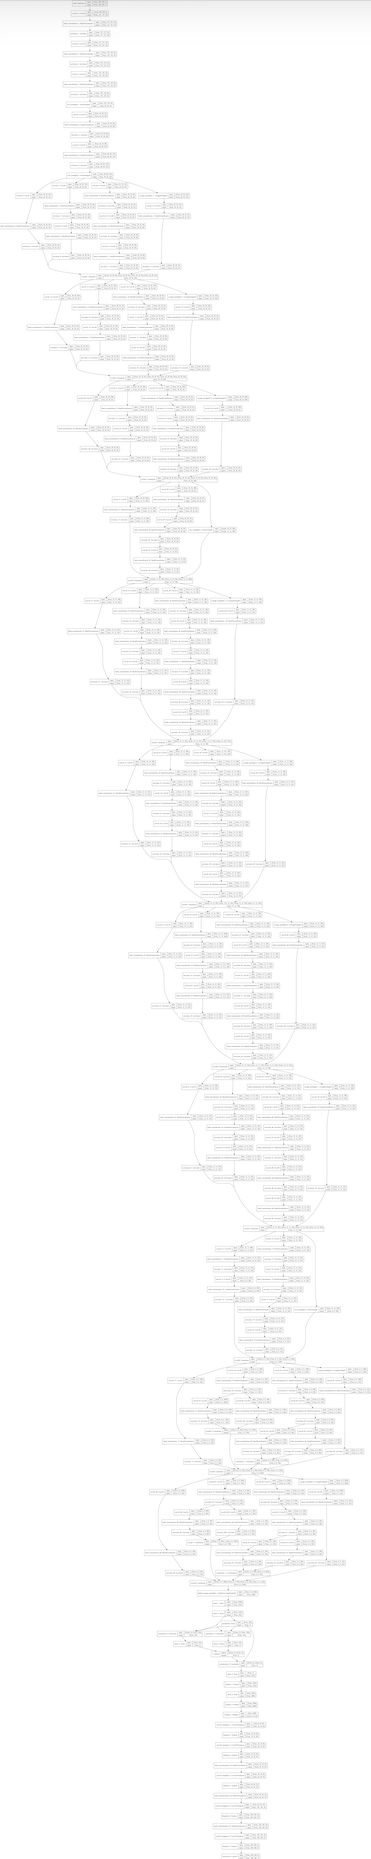
\includegraphics[height=0.9\textheight]{fig/vae_mlp_un_label_v2_tiny}
	\caption{Network architecture of semi-supervised learning model based on VAE with InceptionV3}
	\label{fig:semiVAEmodel}
\end{figure}


\section{GANによる画像生成}
VAE-GANを実装するにあたり,まずはGANによる検体画像の生成を行った.\fig{GANimage}はGANによる画像生成の過程である.\fig{unetae}のAutoEncoderよりGANの方が高精細に生成されていることが分かる.しかし,\fig{vaeresultpicture}に示したVAEで生成された画像よりは不鮮明である.GANを使って高精細な画像を生成することは難しく,安定に生成させるには正確なパラメータチューニングやヒューリスティックが不可欠である.本研究では,ここまでが限界であった.今後のGANの発展に期待したい.

\begin{figure}[H]
	\centering
	
	\begin{minipage}{0.24\columnwidth}
		\centering
		
\includegraphics[clip, width=\linewidth]{fig/generative_adversarial_nets/0000_0000}
		\subcaption{epochs = 0}
		\label{fig:}
	\end{minipage}
	\begin{minipage}{0.24\columnwidth}
		\centering
		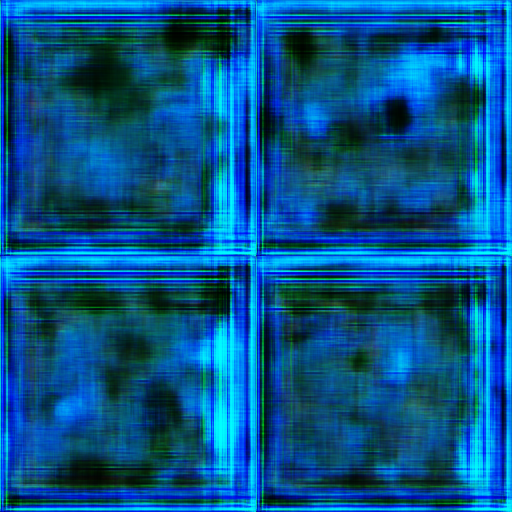
\includegraphics[clip, width=\linewidth]{fig/generative_adversarial_nets/0079_0000}
		\subcaption{epochs = 79}
		\label{fig:}
	\end{minipage}
	\begin{minipage}{0.24\columnwidth}
		\centering
		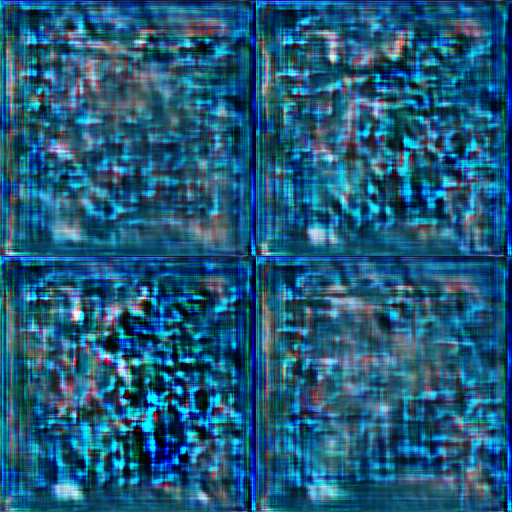
\includegraphics[clip, width=\linewidth]{fig/generative_adversarial_nets/0641_0000}
		\subcaption{epochs = 641}
		\label{fig:}
	\end{minipage}
	\begin{minipage}{0.24\columnwidth}
		\centering
		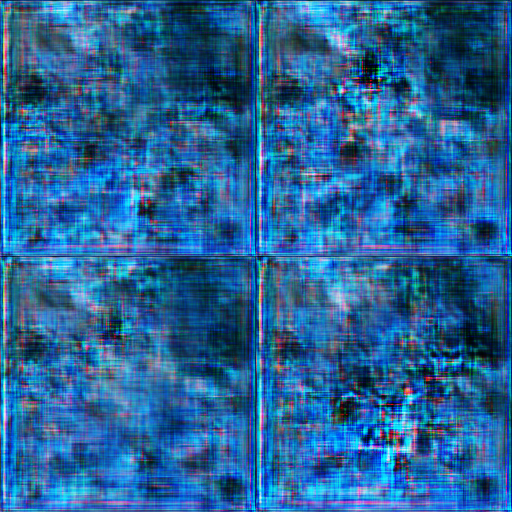
\includegraphics[clip, width=\linewidth]{fig/generative_adversarial_nets/0969_0000}
		\subcaption{epochs = 969}
		\label{fig:}
	\end{minipage}
	\begin{minipage}{0.24\columnwidth}
		\centering
		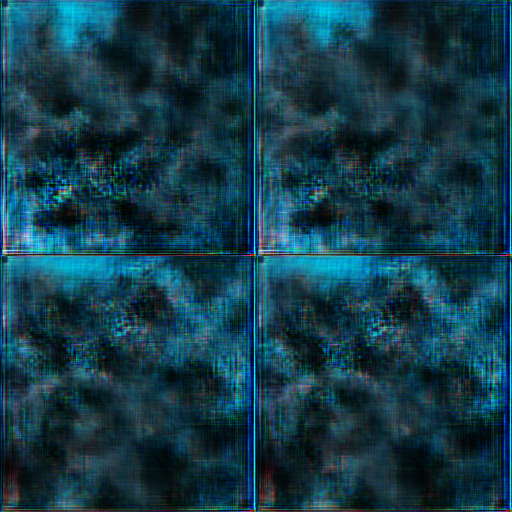
\includegraphics[clip, width=\linewidth]{fig/generative_adversarial_nets/1213_0000}
		\subcaption{epochs = 1213}
		\label{fig:}
	\end{minipage}
	\begin{minipage}{0.24\columnwidth}
		\centering
		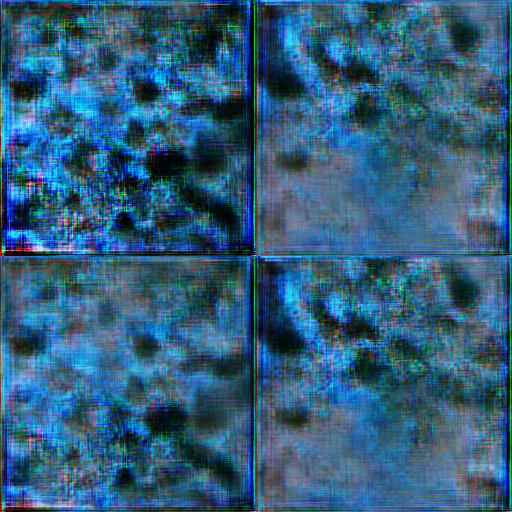
\includegraphics[clip, width=\linewidth]{fig/generative_adversarial_nets/1619_0000}
		\subcaption{epochs = 1619}
		\label{fig:}
	\end{minipage}
	\begin{minipage}{0.24\columnwidth}
		\centering
		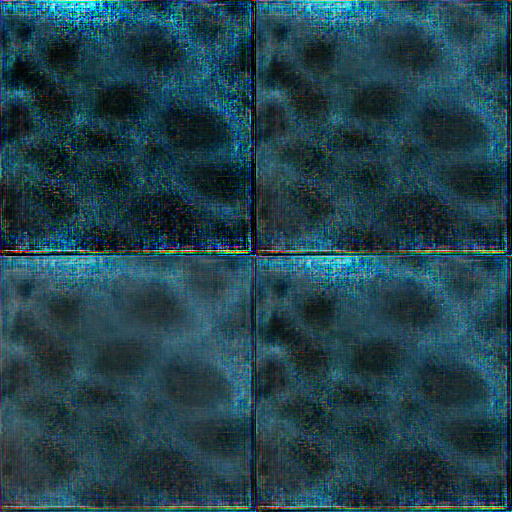
\includegraphics[clip, width=\linewidth]{fig/generative_adversarial_nets/2004_0000}
		\subcaption{epochs = 2004}
		\label{fig:}
	\end{minipage}
	\begin{minipage}{0.24\columnwidth}
		\centering
		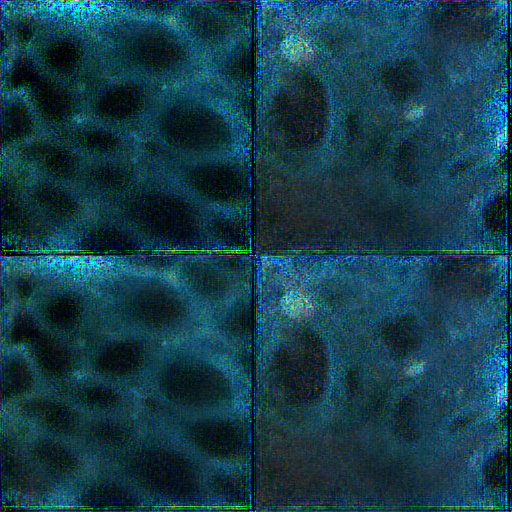
\includegraphics[clip, width=\linewidth]{fig/generative_adversarial_nets/3208_0000}
		\subcaption{epochs = 3208}
		\label{fig:}
	\end{minipage}
	
	\caption{Transition of generated images by GAN}
	\label{fig:GANimage}
	
\end{figure}